\section{User Interface}
\label{sec:ui}

Since we've chosen to use SDL2 as our rendering library, and SDL2 is just a 
microframework used for rendering to a window; we had to create our own GUI 
library. This means that we had to create a way to create and place GUI 
components like panels, buttons and text. This chapter will go in depth on 
how we created our own GUI library and how to use it.

\subsection{Templated UIComponent}
While creating the GUI library, we've used a lot of templating. This was done 
so that we can reuse our templated GUI classes if and when we decide to 
switch to OpenGL. The lowest level GUI class is called the UIComponent, 
which has a couple of template parameters for which rendering engine we're 
using,  the type of data its rendering object (see \cref{sec:rendering-ui} for 
an explanation about how the UIComponents get rendered.) contains, what kind 
of data it returns when rendering and the type of data for its mouse callback 
object (which will be explained in \cref{sec:eventhandling}).

The UIComponent class can be seen in \cref{fig:uicomponent}.

\begin{figure}[H]
\centering
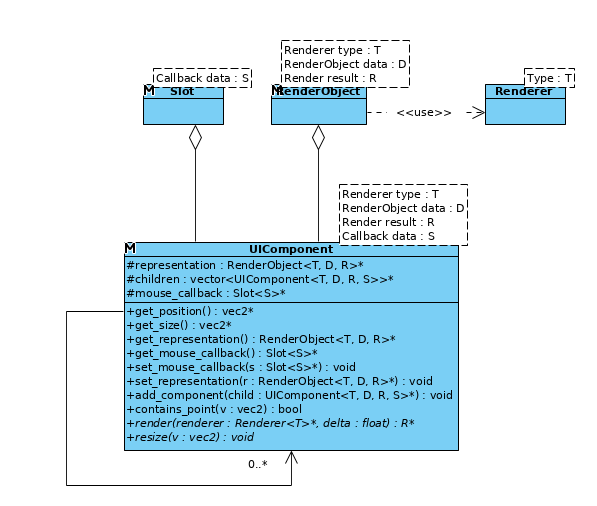
\includegraphics[scale=0.55]{res/ui/uicomponent.png}
\caption{UIComponent class.}\label{fig:uicomponent}
\end{figure}


\subsection{SDL2 GUI implementation}
\label{sec:sdl2gui}

Since we're using SDL2, we've made an implementation of the UIComponent class
 with the following template arguments:
\begin{itemize}
\item T = SDL\_Renderer (Rendering engine used by SDL2)
\item D = sdl\_data (a data structure)
\item R = SDL\_Texture (SDL2's texture structure)
\item S = sdl\_mouse\_event\_data (data used by the mouse callback object)
\end{itemize}

You can also create custom SDL\_UIComponent by inheriting from the 
SDL\_UIComponent class as shown in \cref{fig:sdluicomponent-inherit}. You can 
also use a custom struct that inherits from sdl\_data if your class' 
rendering object uses a different data type. For example, the SDLButton 
rendering object uses a struct that has been derived from the sdl\_data 
struct, which can be seen in \cref{lst:sdlbuttondata}.

\begin{figure}[!htb]
\centering
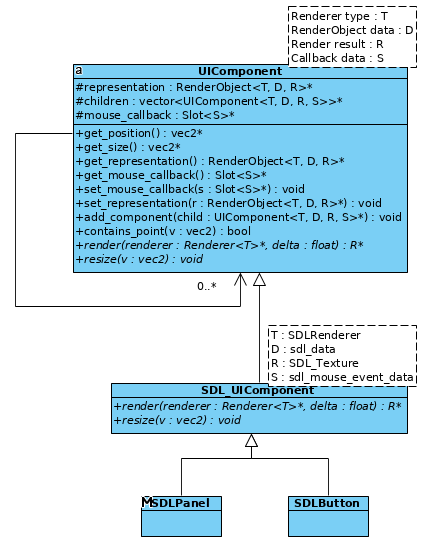
\includegraphics[scale=0.75]{res/ui/sdluicomponent-inherit.png}
\caption{SDL\_UIComponent class inheritance.}\label{fig:sdluicomponent-inherit}
\end{figure}

